\subsection{Utente non autenticato}
\subsubsection{Panoramica utente non autenticato}
\begin{figure}[H]
\centering
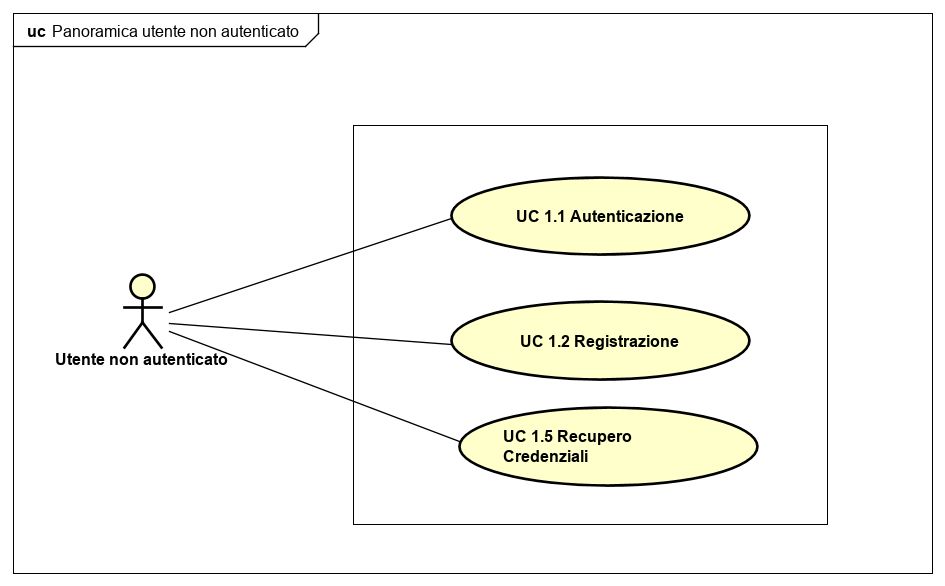
\includegraphics[width=17cm]{img/UC1.png} 
\caption{Panoramica utente non autenticato}\label{fig:1}
\end{figure}


\subsubsection{UC 1.1 - Autenticazione}

\begin{figure}[H]
\centering
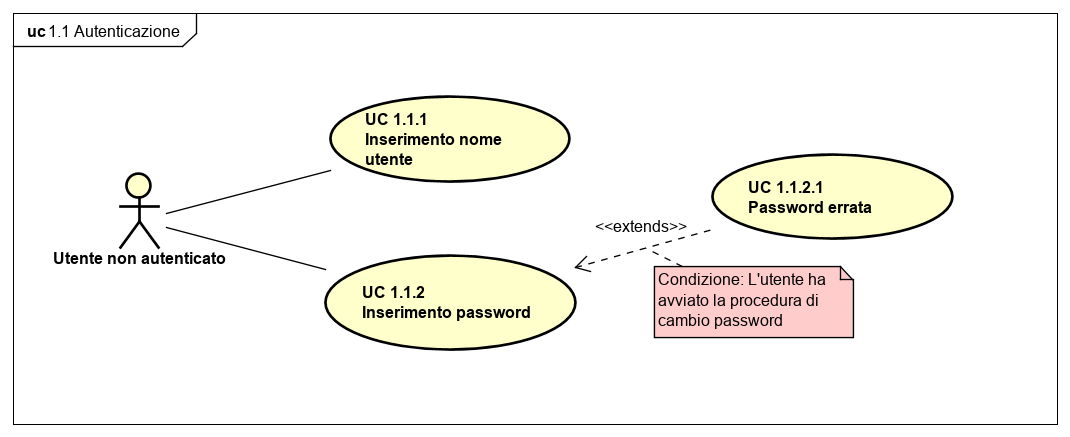
\includegraphics[width=17cm]{img/UC11.png} 
\caption{Caso d'uso UC 1.1}
\end{figure}

\begin{itemize}
\item[•]\textbf{Attori}: Utente non autenticato;
\item[•]\textbf{Descrizione}:  l’utente non identificato inserisce username e password e si autentica accedendo alla dashboard;
\item[•]\textbf{Precondizione}: l’utente non è autenticato;
\item[•]\textbf{Postcondizione}: l’utente viene autenticato all’interno del sistema;
\item[•]\textbf{Flusso degli eventi principale}:
\begin{enumerate}
\item UC 1.1.1 - Inserimento nome utente;
\item UC 1.1.2 - Inserimento password;
\item UC 1.1.3 - Reset password.
\end{enumerate}
\item[•]\textbf{Estensioni}:
\begin{enumerate}
\item UC 1.1.2.1 - Visualizazzione messaggio d'errore del nome utente o password sbagliata.

\end{enumerate}
\end{itemize}

\subsubsection{UC 1.1.1 - Inserimento nome utente}
\begin{itemize}
\item[•]\textbf{Attori}: Utente non autenticato;
\item[•]\textbf{Descrizione}: l’utente inserisce un nome utente durante la registrazione;
\item[•]\textbf{Precondizione}: l’utente non è autenticato;
\item[•]\textbf{Postcondizione}: l’utente ha inserito il proprio nome utente.
\end{itemize}

\subsubsection{UC 1.1.2 - Inserimento password}
\begin{itemize}
\item[•]\textbf{Attori}: Utente non autenticato;
\item[•]\textbf{Descrizione}: l’utente inserisce una password;
\item[•]\textbf{Precondizione}: l'utente non è autenticato;
\item[•]\textbf{Postcondizione}: l'utente ha inserito la propria password.
\end{itemize}
\subsubsection{UC 1.1.2.1  - Visualizazzione messaggio d'errore del nome utente o password sbagliata}
\begin{itemize}
\item[•]\textbf{Attori}: Utente non autenticato;
\item[•]\textbf{Descrizione}: l’utente inserisce le credenziali sbagliate;
\item[•]\textbf{Precondizione}: l'utente non è autenticato;
\item[•]\textbf{Postcondizione}: l'utente riceve il messaggio d'erorre.
\end{itemize}

\subsubsection{UC 1.1.3 - Reset password}
\begin{itemize}
	\item[•]\textbf{Attori}: Utente non autenticato;
	\item[•]\textbf{Descrizione}: l’utente inserisce i propri dati in maniera errata e avvia iter per il reset password;
	\item[•]\textbf{Precondizione}: l’utente non è autenticato;
	\item[•]\textbf{Postcondizione}: l’utente ha inviato la richiesta di reset password.
\end{itemize}

\subsubsection{UC 1.2 - Registrazione utente}
\begin{figure}[H]
	\centering
	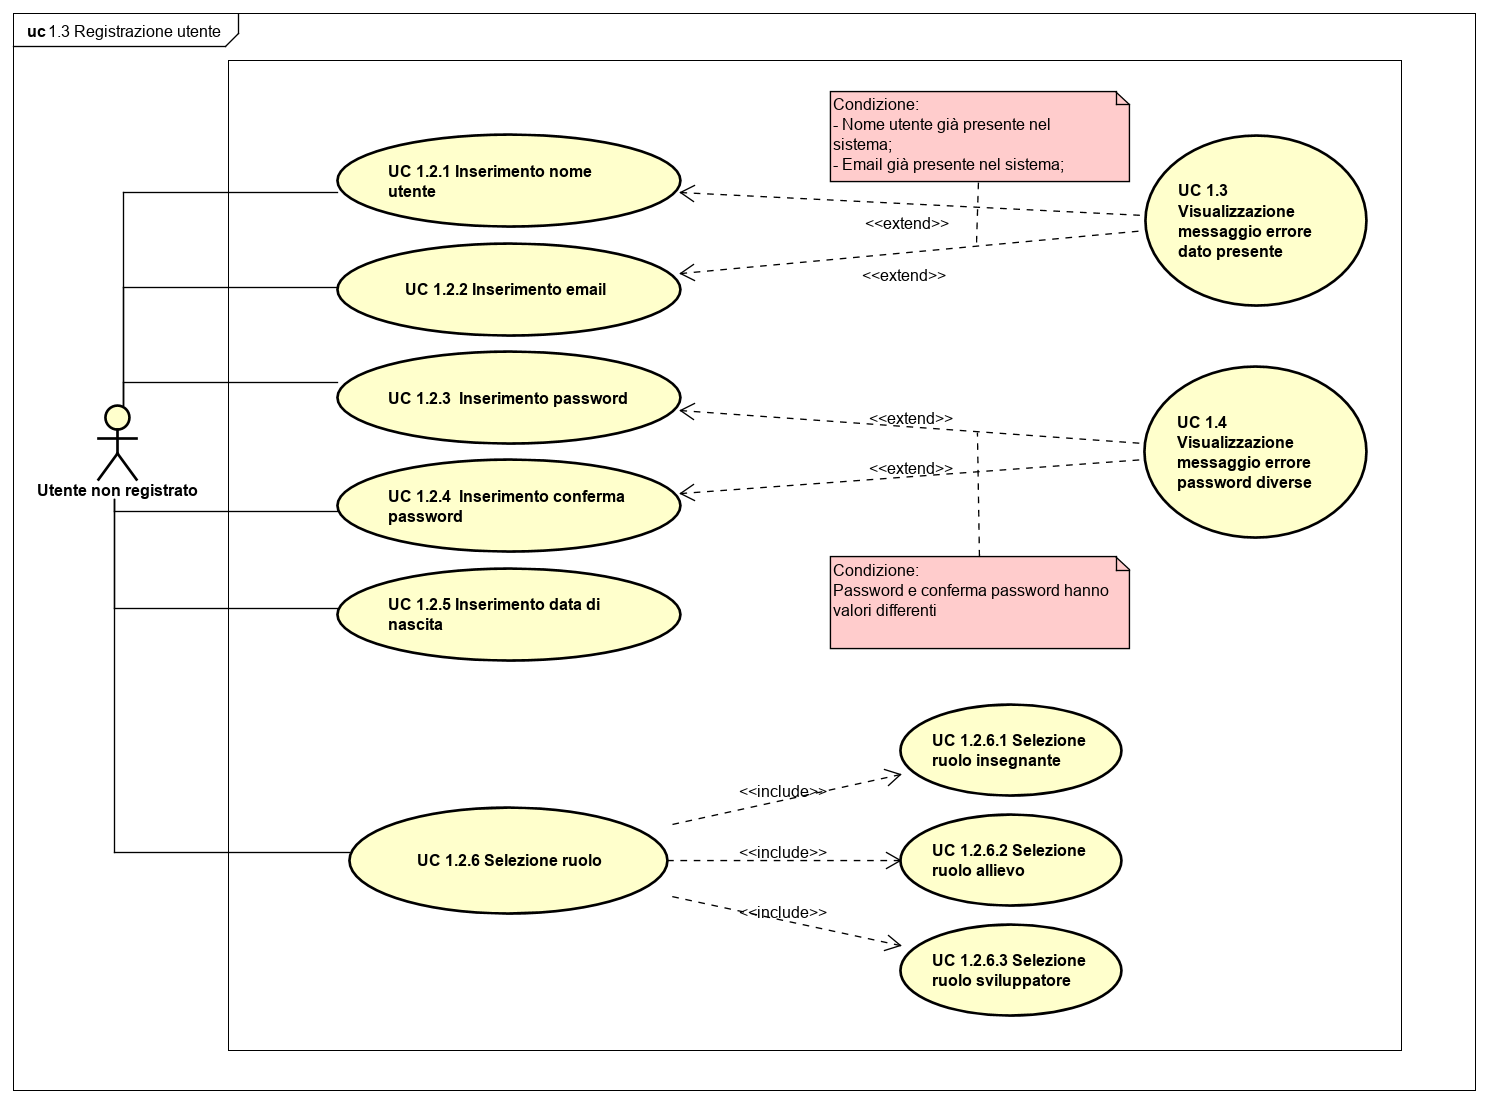
\includegraphics[width=17cm]{img/UC12.png} 
	\caption{Caso d'uso UC 1.2}\label{fig:12}
\end{figure}
\begin{itemize}
	\item[•]\textbf{Attori}: Utente non registrato;
	\item[•]\textbf{Descrizione}: l'utente non registrato compila il modulo di registrazione al fine di poter accedere al sistema;
	\item[•]\textbf{Precondizione}: l'utente non è registrato;
	\item[•]\textbf{Postcondizione}: l'utente si è registrato e può quindi accedere al sistema;
	\item[•]\textbf{Flusso degli eventi principale}:
	\begin{enumerate}
		\item UC 1.2.1 - Inserimento nome utente;
		\item UC 1.2.2 - Inserimento email;
		\item UC 1.2.3 - Inserimento password;
		\item UC 1.2.4 - Inserimento conferma password;
		\item UC 1.2.5 - Inserimento data di nascita;
		\item UC 1.2.6 - Selezione ruolo.
	\end{enumerate}
	\item[•]\textbf{Estensioni}:
	\begin{enumerate}
		\item UC 1.3 - Visualizzazione messaggio errore dato presente;
		\item UC 1.4 - Visualizzazione messaggio errore password diverse.
	\end{enumerate}
\end{itemize}

\subsubsection{UC 1.2.1 - Inserimento nome utente}
\begin{itemize}
	\item[•]\textbf{Attori}: Utente non registrato;
	\item[•]\textbf{Descrizione}: l'utente inserisce un nome utente durante la registrazione;
	\item[•]\textbf{Precondizione}: l'utente non è registrato e il nome utente non è definito;
	\item[•]\textbf{Postcondizione}: l'utente ha inserito un nome utente;
	\item[•] \textbf{Estensioni}:
	\begin{enumerate}
		\item UC 1.3 - Visualizzazione messaggio errore dato presente.
	\end{enumerate}
\end{itemize}

\subsubsection{UC 1.2.2 - Inserimento email}
\begin{itemize}
	\item[•]\textbf{Attori}: Utente non registrato;
	\item[•]\textbf{Descrizione}: l'utente inserisce la sua email durante la registrazione;
	\item[•]\textbf{Precondizione}: l'utente non è registrato e la email non è definita;
	\item[•]\textbf{Postcondizione}: l'utente ha inserito la propria email;
	\item[•] \textbf{Estensioni}:
		\begin{enumerate}
		\item UC 1.3 - Visualizzazione messaggio errore dato presente.
	\end{enumerate}
\end{itemize}

\subsubsection{UC 1.2.3 - Inserimento password}
\begin{itemize}
	\item[•]\textbf{Attori}: Utente non registrato;
	\item[•]\textbf{Descrizione}: l'utente inserisce una password durante procedura di registrazione;
	\item[•]\textbf{Precondizione}: l'utente non è registrato e la password non è definita;
	\item[•]\textbf{Postcondizione}: l'utente ha inserito una password;
	\item[•] \textbf{Estensioni}:
	\begin{enumerate}
		\item UC 1.4 - Visualizzazione messaggio errore password diverse.
	\end{enumerate}
\end{itemize}

\subsubsection{UC 1.2.4 - Inserimento conferma password}
\begin{itemize}
	\item[•]\textbf{Attori}: Utente non registrato;
	\item[•]\textbf{Descrizione}: l'utente inserisce la conferma della password durante la registrazione;
	\item[•]\textbf{Precondizione}: l'utente non è registrato e la conferma password non è definita;
	\item[•]\textbf{Postcondizione}: l'utente ha inserito la conferma della password;
	\item[•] \textbf{Estensioni}:
		\begin{enumerate}
		\item UC 1.4 - Visualizzazione messaggio errore password diverse.
	\end{enumerate}
\end{itemize}

\subsubsection{UC 1.2.5 - Inserimento data di nascita}
\begin{itemize}
	\item[•]\textbf{Attori}: Utente non registrato;
	\item[•]\textbf{Descrizione}: l'utente inserisce la sua data di nascita durante la registrazione;
	\item[•]\textbf{Precondizione}: l'utente non è registrato e la data di nascita non è definita;
	\item[•]\textbf{Postcondizione}: l'utente ha inserito la sua data di nascita.
\end{itemize}

\subsubsection{UC 1.2.6 - Selezione ruolo}
\begin{itemize}
	\item[•]\textbf{Attori}: Utente non registrato;
	\item[•]\textbf{Descrizione}: l'utente seleziona il ruolo che vorrebbe ricoprire all'interno dell'applicativo;
	\item[•]\textbf{Precondizione}: l'utente non è registrato e il ruolo non è definito;
	\item[•]\textbf{Postcondizione}: l'utente ha inserito il ruolo desiderato.
\end{itemize}

\subsubsection{UC 1.3 - Visualizzazione messaggio errore dato presente}
\begin{itemize}
	\item[•]\textbf{Attori}: Utente non registrato;
	\item[•]\textbf{Descrizione}: l'utente non registrato visualizza un messaggio di errore relativo all'inserimento
	di un dato già presente nel sistema;
	\item[•]\textbf{Precondizione}: l'utente non registrato sta completando la procedura di registrazione;
	\item[•]\textbf{Postcondizione}: l'utente visualizza un messaggio di errore relativo all'inserimento di un valore già presente nel sistema;
	\item[•]\textbf{Flusso degli eventi principale}: l'utente inserisce una email o un nome utente già presente nel sistema, pertanto riceve un messaggio di errore.
\end{itemize}

\subsubsection{UC 1.4 - Visualizzazione messaggio errore password diverse}
\begin{itemize}
	\item[•]\textbf{Attori}: Utente non registrato;
	\item[•]\textbf{Descrizione}: l'utente non registrato visualizza un messaggio che comunica che i valori della password e di conferma password sono tra loro diversi;
	\item[•]\textbf{Precondizione}: l'utente non registrato ha inserito la password e la conferma password con valori differenti;
	\item[•]\textbf{Postcondizione}: l'utente visualizza un messaggio di errore relativo all'inserimento di password e conferma password con valori diversi;
	\item[•]\textbf{Flusso degli eventi principale}: l'utente inserisce password e conferma password con valori diversi, pertanto riceve un messaggio di errore.
\end{itemize}